\documentclass[10pt,aspectratio=169,serif]{beamer}

\usepackage[fontset=none, scheme=plain]{ctex}
\IfFontExistsTF{Songti SC}{%
	\setCJKmainfont{Songti SC}[AutoFakeSlant=0.2]%
	\setCJKsansfont{Songti SC}[AutoFakeSlant=0.2]%
}{%
	\setCJKmainfont{FandolSong-Regular}[Extension=.otf,BoldFont=FandolSong-Bold,AutoFakeSlant=0.2]%
	\setCJKsansfont{FandolSong-Regular}[Extension=.otf,BoldFont=FandolSong-Bold]%
}
\usepackage{amsmath,amssymb,graphicx,tikz,booktabs,multicol,calligra}
\usepackage{pgfplots}
\pgfplotsset{compat=1.18}
\usepackage{tcolorbox}
\tcbuselibrary{skins}
\usepackage{XyygU}
\usepackage{caption}
\captionsetup[figure]{name=图,labelsep=period}

\usetikzlibrary{arrows.meta,positioning,calc}

\setlength{\abovedisplayskip}{0pt plus 2pt minus 2pt}
\setlength{\belowdisplayskip}{0pt plus 2pt minus 2pt}

\title[4.5 函数的应用（二）练习]{4.5 函数的应用（二）（练习）}
\subtitle{函数零点 \& 二分法 \& 函数模型的应用}
\author{}
\institute{}
\date{2026-10-16}

\begin{document}

\begin{frame}
  \titlepage
\end{frame}

% ============================================================
% 练习（二分法）第1题
% ============================================================
\begin{frame}[t]{练习1：二分法求三次函数零点}
\textbf{1.} 借助信息技术，用二分法求函数
\[
f(x)=x^{3}+1.1x^{2}+0.9x-1.4
\]
在区间 $(0,1)$ 内零点的近似值（精确度为 $0.1$）。
\end{frame}

\begin{frame}[t]{练习1 解答}
\vspace{-1em}
\begin{tcolorbox}[colback=orange!10,colframe=orange,title=\textbf{解}]
$f(0)=-1.4<0$，$f(1)=1+1.1+0.9-1.4=1.6>0$，故零点 $x_{0}\in(0,1)$。
\smallskip
\begin{enumerate}
  \item 取中点 $x_{1}=0.5$，$f(0.5)=-0.55<0$，$\Rightarrow x_{0}\in(0.5,1)$；
  \item 取中点 $x_{2}=0.75$，$f(0.75)\approx 0.316>0$，$\Rightarrow x_{0}\in(0.5,0.75)$；
  \item 取中点 $x_{3}=0.625$，$f(0.625)\approx -0.164<0$，$\Rightarrow x_{0}\in(0.625,0.75)$；
  \item 取中点 $x_{4}=0.6875$，$f(0.6875)\approx 0.064>0$，$\Rightarrow x_{0}\in(0.625,0.6875)$。
\end{enumerate}
因为 $|0.6875-0.625|=0.0625<0.1$，满足精确度要求。
\smallskip
\textbf{所以零点近似值可取 } $\alert{x_{0}\approx 0.66}$\textbf{（或取区间端点 $0.625$、$0.6875$ 均可）}。
\end{tcolorbox}
\end{frame}

\begin{frame}[t]{练习1 函数图象}
\begin{center}
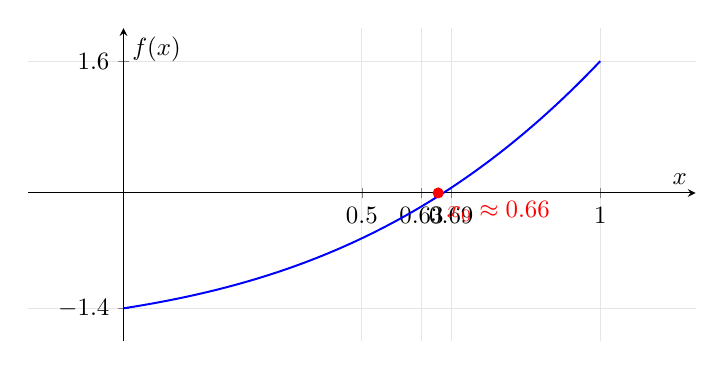
\begin{tikzpicture}[scale=0.9]
\begin{axis}[
    width=11cm, height=6cm,
    axis lines=middle,
    xlabel=$x$, ylabel=$f(x)$,
    xmin=-0.2, xmax=1.2, ymin=-1.8, ymax=2,
    xtick={0,0.5,0.625,0.6875,1},
    ytick={-1.4,0,1.6},
    grid=major, grid style={gray!20},
]
\addplot[thick,blue,domain=0:1,samples=100] {x^3+1.1*x^2+0.9*x-1.4};
\addplot[only marks,mark=*,mark size=2pt,red] coordinates {(0.66,0)};
\node[red,below right] at (axis cs:0.66,0) {$x_{0}\approx0.66$};
\end{axis}
\end{tikzpicture}
\end{center}
\end{frame}

% ============================================================
% 练习（二分法）第2题
% ============================================================
\begin{frame}[t]{练习2：二分法求对数方程近似解}
\textbf{2.} 借助信息技术，用二分法求方程
\[
x=3-\lg x
\]
在区间 $(2,3)$ 内的近似解（精确度为 $0.1$）。
\end{frame}

\begin{frame}[t]{练习2 解答}
\vspace{-1em}
\begin{tcolorbox}[colback=orange!10,colframe=orange,title=\textbf{解}]
原方程即 $f(x)=x+\lg x-3=0$。
$f(2)=2+\lg 2-3\approx -0.699<0$，$f(3)=3+\lg 3-3\approx 0.477>0$，故 $x_{0}\in(2,3)$。
\smallskip
\begin{enumerate}
  \item $x_{1}=2.5$，$f(2.5)\approx -0.102<0$ $\Rightarrow x_{0}\in(2.5,3)$；
  \item $x_{2}=2.75$，$f(2.75)\approx 0.189>0$ $\Rightarrow x_{0}\in(2.5,2.75)$；
  \item $x_{3}=2.625$，$f(2.625)\approx 0.044>0$ $\Rightarrow x_{0}\in(2.5,2.625)$；
  \item $x_{4}=2.5625$，$f(2.5625)\approx -0.029<0$ $\Rightarrow x_{0}\in(2.5625,2.625)$。
\end{enumerate}
$|2.625-2.5625|=0.0625<0.1$，满足精确度。
\smallskip
\textbf{原方程近似解为 } $\alert{x\approx 2.59}$\textbf{（或取 $2.56$、$2.63$）}。
\end{tcolorbox}
\end{frame}

% ============================================================
% 练习（函数模型）第1题：世界人口
% ============================================================
\begin{frame}[t]{练习3：世界人口的马尔萨斯模型}
\textbf{1.} 已知 $1650$ 年世界人口为 $5$ 亿，当时人口年增长率为 $0.3\%$；$1970$ 年世界人口为 $36$ 亿，当时人口年增长率为 $2.1\%$。
\begin{enumerate}
  \item 用马尔萨斯人口模型计算：什么时候世界人口是 $1650$ 年的 $2$ 倍？什么时候世界人口是 $1970$ 年的 $2$ 倍？
  \item 实际上，$1850$ 年以前世界人口就超过了 $10$ 亿；而 $2004$ 年世界人口还没有达到 $72$ 亿。你对同样的模型得出的两个结果有何看法？
\end{enumerate}
\end{frame}

\begin{frame}[t]{练习3 解答 (1)}
\begin{tcolorbox}[colback=orange!10,colframe=orange,title=\textbf{解 (1)}]
马尔萨斯模型 $y=y_{0}e^{rt}$。
\smallskip
\textbf{第一阶段：} $y_{0}=5$ 亿，$r=0.003$。人口翻倍即 $y=10$：
\[
10=5e^{0.003t}\ \Rightarrow\ e^{0.003t}=2\ \Rightarrow\ t=\frac{\ln 2}{0.003}\approx 231.
\]
即 $1650+231\approx \alert{1881}$ 年世界人口达到 $10$ 亿。
\smallskip
\textbf{第二阶段：} $y_{0}=36$ 亿，$r=0.021$。人口翻倍即 $y=72$：
\[
72=36e^{0.021t}\ \Rightarrow\ t=\frac{\ln 2}{0.021}\approx 33.
\]
即 $1970+33\approx \alert{2003}$ 年世界人口达到 $72$ 亿。
\end{tcolorbox}
\end{frame}

\begin{frame}[t]{练习3 解答 (2)}
\begin{tcolorbox}[colback=orange!10,colframe=orange,title=\textbf{解 (2)：模型评价}]
\begin{itemize}
  \item 模型预测 $1881$ 年人口才翻倍到 $10$ 亿，但实际 $1850$ 年前已超过 $10$ 亿，说明早期实际人口增长比 $0.3\%$ 模型预测的要快；
  \item 模型预测 $2003$ 年人口达到 $72$ 亿，但 $2004$ 年实际尚未达到，说明后期人口增长率放缓（计划生育、战争、经济因素等）；
  \item \textbf{结论：} 马尔萨斯模型只在较短时期、较稳定条件下近似成立。实际人口受政策、经济、战争、疾病等多种因素影响，不能简单用一个指数模型长期外推。使用函数模型时应注意\alert{模型的适用条件和时间范围}。
\end{itemize}
\end{tcolorbox}
\end{frame}

% ============================================================
% 练习（函数模型）第2题：野兔繁殖
% ============================================================
\begin{frame}[t]{练习4：野兔繁殖}
\textbf{2.} 在一段时间内，某地的野兔快速繁殖，野兔总只数的倍增期为 $21$ 个月，那么 $1$ 万只野兔增长到 $1$ 亿只野兔大约需要多少年？
\end{frame}

\begin{frame}[t]{练习4 解答}
\begin{tcolorbox}[colback=orange!10,colframe=orange,title=\textbf{解}]
设经过 $n$ 个倍增期，则野兔数量为 $y=10^{4}\cdot 2^{n}$。
要求 $y=10^{8}$：
\[
10^{4}\cdot 2^{n}=10^{8}\ \Rightarrow\ 2^{n}=10^{4}.
\]
\[
n=\log_{2}10^{4}=\frac{\lg 10^{4}}{\lg 2}=\frac{4}{0.3010}\approx 13.29.
\]
所需时间：
\[
t=13.29\times 21\ \text{个月}\approx 279\ \text{个月}\approx \alert{23.3\ \text{年}}.
\]
\smallskip
\textbf{即约需 $23$ 年}（指数增长惊人，体现了\alert{指数爆炸}现象）。
\end{tcolorbox}
\end{frame}

% ============================================================
% 练习（函数模型）第3题：碳14 二里头
% ============================================================
\begin{frame}[t]{练习5：碳14 测年——二里头遗址}
\textbf{3.} $1959$ 年，考古学家在河南洛阳偃师市区二里头村发掘出了一批古建筑群，从其中的某样本中检测出碳 $14$ 的残余量约为初始量的 $62.76\%$，能否以此推断二里头遗址大概是什么年代的？
\end{frame}

\begin{frame}[t]{练习5 解答}
\begin{tcolorbox}[colback=orange!10,colframe=orange,title=\textbf{解}]
碳 $14$ 半衰期为 $5730$ 年，残余量模型：
\[
y=k\left(\tfrac12\right)^{x/5730}.
\]
由题意 $\left(\tfrac12\right)^{x/5730}=0.6276$：
\[
x=5730\cdot \log_{1/2}0.6276
   =5730\cdot\frac{\ln 0.6276}{\ln 0.5}
   \approx 5730\times 0.672\approx 3852\ \text{年}.
\]
\smallskip
即样本距 $1959$ 年约 $3852$ 年：
\[
1959-3852\approx -1893.
\]
\textbf{推断二里头遗址大约建于 }$\alert{\text{公元前 }1900\text{ 年左右}}$\textbf{，与夏代纪年基本吻合。}
\end{tcolorbox}
\end{frame}

% ============================================================
% 练习（函数模型选择）第1题：传染病
% ============================================================
\begin{frame}[t]{练习6：传染病模型的选择}
\textbf{1.} 某地今年 $1,2,3$ 月患某种传染病的人数分别为 $52,61,68$。为了预测以后各月的患病人数，甲选择了模型 $y=ax^{2}+bx+c$，乙选择了模型 $y=pq^{x}+r$，其中 $y$ 为患病人数，$x$ 为月份数。结果 $4,5,6$ 月份患病人数分别为 $74,78,83$，你认为谁选择的模型更符合实际？
\end{frame}

\begin{frame}[t]{练习6 解答：甲的二次模型}
\begin{tcolorbox}[colback=orange!10,colframe=orange,title=\textbf{解：甲模型 $y=ax^{2}+bx+c$}]
用前 3 个月数据：
\[
\begin{cases}
a+b+c=52\\
4a+2b+c=61\\
9a+3b+c=68
\end{cases}
\Rightarrow a=-1,\ b=12,\ c=41.
\]
\textbf{预测：}
\[
y=-x^{2}+12x+41.
\]
\begin{tabular}{l|ccc}
月份 $x$ & 4 & 5 & 6\\ \hline
预测值 & 73 & 76 & 77\\
实际值 & 74 & 78 & 83\\
误差 & 1 & 2 & 6
\end{tabular}
\end{tcolorbox}
\end{frame}

\begin{frame}[t]{练习6 解答：乙的指数模型}
\begin{tcolorbox}[colback=orange!10,colframe=orange,title=\textbf{解：乙模型 $y=pq^{x}+r$}]
用前 3 个月数据，两式相除得 $q=\dfrac{7}{9}$，进而：
\[
pq=-\frac{81}{2},\quad r=\frac{745}{8}\approx 92.5.
\]
\textbf{预测：}
\[
y=-40.5\left(\tfrac{7}{9}\right)^{x}+92.5.
\]
\begin{tabular}{l|ccc}
月份 $x$ & 4 & 5 & 6\\ \hline
预测值 & 73.4 & 77.7 & 81.0\\
实际值 & 74 & 78 & 83\\
误差 & 0.6 & 0.3 & 2.0
\end{tabular}
\smallskip
\textbf{比较：} 甲模型误差和 $=1+2+6=9$；乙模型误差和 $\approx 0.6+0.3+2.0=2.9$。
\textbf{乙模型误差更小，故 }$\alert{\text{乙选择的模型更符合实际}}$。
\end{tcolorbox}
\end{frame}

% ============================================================
% 练习（函数模型选择）第2题：肉鸡与人口
% ============================================================
\begin{frame}[t]{练习7：肉鸡产量与人口}
\textbf{2.} $2008\sim 2018$ 年，某地上市肉鸡数量（吨）与人口数（万）如下：
\smallskip
\begin{tabular}{l|ccccccccccc}
年份 & 2008&2009&2010&2011&2012&2013&2014&2015&2016&2017&2018\\ \hline
肉鸡/吨 &7690&7850&8000&8150&8310&8460&8620&8770&8920&9080&9230\\
人口/万 &100.0&101.2&102.4&103.6&104.9&106.1&107.4&108.7&110.0&111.3&112.7
\end{tabular}
\begin{enumerate}
  \item 分别求出能近似反映两组数据变化规律的函数；
  \item 如果 $2017$ 年该地肉鸡基本能满足本地需求，那么 $2018$ 年是否能满足市场需求？
  \item 对该地 $2018$ 年后肉鸡市场发展有何建议？
\end{enumerate}
\end{frame}

\begin{frame}[t]{练习7 解答 (1)：建立线性模型}
\begin{tcolorbox}[colback=orange!10,colframe=orange,title=\textbf{解 (1)}]
设 $x$ 为距 $2008$ 年的年数（$x=0,1,\dots,10$）。两组数据均近似线性增长。
\smallskip
\textbf{肉鸡产量：} 端点 $(0,7690)$、$(10,9230)$，斜率 $k_{1}=\dfrac{9230-7690}{10}=154$：
\[
y_{1}=7690+154x.
\]
\textbf{人口数：} 端点 $(0,100.0)$、$(10,112.7)$，斜率 $k_{2}=\dfrac{112.7-100.0}{10}=1.27$：
\[
y_{2}=100.0+1.27x.
\]
（模型与表中数据误差在 $1\%$ 以内。）
\end{tcolorbox}
\end{frame}

\begin{frame}[t]{练习7 解答 (2)(3)}
\begin{tcolorbox}[colback=orange!10,colframe=orange,title=\textbf{解 (2)(3)}]
\textbf{(2)} 增长率比较：
\[
\text{肉鸡增长率}=\frac{9230-9080}{9080}\approx 1.65\%,\qquad
\text{人口增长率}=\frac{112.7-111.3}{111.3}\approx 1.26\%.
\]
肉鸡产量增长率高于人口增长率，人均肉鸡占有量略增。
\textbf{故 2018 年仍能满足本地需求。}
\smallskip
\textbf{(3) 建议：}
\begin{itemize}
  \item 肉鸡产量年增约 $1.6\%$，人口年增约 $1.3\%$，产能略大于需求增长；
  \item 可适当拓展外地市场、发展深加工；
  \item 警惕产能过剩，避免盲目扩大养殖规模。
\end{itemize}
\end{tcolorbox}
\end{frame}

\begin{frame}[c]
  \begin{center}
    {\Huge\calligra Thanks!}
  \end{center}
\end{frame}

\end{document}
